%%% Preamble
\documentclass[paper=letterpaper, fontsize=11pt]{scrartcl}
\usepackage[T1]{fontenc}
\usepackage{fourier} % Uses Adobe Utopia font by default
%\usepackage{eucal} % Better mathcal fonts
\DeclareMathAlphabet{\mathcal}{OMS}{cmsy}{m}{n} % Reset mathcal fonts to default
\usepackage{hyperref}
\usepackage[margin=1in]{geometry}
\usepackage{float}
\usepackage[font=small,labelfont=bf]{caption}
\setcapindent{0pt}
%\usepackage[font=small,labelfont=bf]{subcaption}
%\usepackage{natbib}

\usepackage[english]{babel} % English language/hyphenation
\usepackage[protrusion=true,expansion=true]{microtype}

% Math packages
\usepackage{physics} % physics notation/commands
\usepackage{amsmath,amsfonts,amsthm,amssymb} %math,fonts,theorems,symbols
\usepackage{gensymb, cancel}

% Graphics packages
\usepackage[pdftex]{graphicx}	
\usepackage{xcolor}

% Hyperlink package
\usepackage{url}

%%% Custom sectioning
\usepackage{sectsty}
\allsectionsfont{\centering \normalfont\scshape}

%%% Custom headers/footers (fancyhdr package)
\usepackage{fancyhdr}
\pagestyle{fancyplain}
%\fancyhead{}									% No page header
\fancyhead[R]{\thepage}
\fancyhead[L]{\small{Exoplanet Transit Classification
and \\
Parameterization using Recurrent Neural Networks}}
\fancyfoot[L]{\small{Chetan Chawla}}
\fancyfoot[C]{}					
\fancyfoot[R]{\small{\today}}			

\renewcommand{\headrulewidth}{1pt}			% Remove header underlines
\renewcommand{\footrulewidth}{0pt}				% Remove footer underlines
\setlength{\headheight}{2pt}


%%% Equation and float numbering
\numberwithin{equation}{section}		% Equationnumbering: section.eq#
\numberwithin{figure}{section}			% Figurenumbering: section.fig#
\numberwithin{table}{section}			% Tablenumbering: section.tab#


%%% Maketitle metadata
\newcommand{\horrule}[1]{\rule{\linewidth}{#1}} 	% Horizontal rule

\title{
		%\vspace{-1in} 	
		\usefont{OT1}{bch}{b}{n}
		\normalfont \normalsize \textsc{Intro To Astro 2020 - Final Project Proposal} \\ [25pt]
		\horrule{0.5pt} \\[0.4cm]
		\huge Exoplanet Transit Classification and Parameterization using Recurrent Neural Networks \\
		\horrule{2pt} \\[0.5cm]
}

\author{
	\normalfont 				\normalsize
        Chetan Chawla	\\		\normalsize
        \today
}
\date{}


%%% Begin document
\begin{document}
\maketitle

\section{Introduction}
% What will be the final product of this work? (thesis, publication, a new research tool, etc.)

%What do you want to find out? What don’t we already know? 

%Why are you doing this research? Why should we care? (Often, this is a new intriguing result that raises a new question to be investigated. Tie it back to society, the real world.)

%What are the broader impacts of this research to the field, society?


A huge amount of data is produced by space based Telescopes, such as, Kepler Space Telescope and TESS (Transiting Exoplanet Survey Satellite), and even wider amounts of data is expected to be produced by upcoming missions like ESA's PLATO (PLAnetary Transits and Oscillations of stars) and the ARIEL (Atmospheric Remote-sensing Infrared Exoplanet Large-survey). These transit telescopes aim to find extra-solar planets (exoplanets) which could potentially harbour intelligent life. With the volume and diversity of transit data being recorded, there is a strong need for methods that can systematically detect and vet transiting exoplanets, separate them from Astrophysical False Positives, help in parameterization of the detected planets such as it's radius and reduce the human intervention in doing so.\\

Kepler pipeline employs vetting systems, such as Decision Tree based Robovetter \cite{robovetter} and Machine Learning (Random Forest) based Autovetter \cite{autovetter} to classify the transit events as Planet Candidate (PC), Astrophysical False Positive (AFP) or Non Transiting Phenomenon (NTP). However, in these methods, heuristics are explicitly defined by humans. The more recent methods explore the use of Deep Learning, a subset of Machine Learning which uses sub-units called Neurons connected over several computational layers to learn the heuristics from data automatically, for vetting exoplanetary transits. Some examples of these are Astronet \cite{astronet}, which uses a disjoint 1-Dimensional Convolutional Neural Network (CNN), and Exonet \cite{exonet}, which improves on Astronet by factoring in scientific domain knowledge. The 1-D CNN incorporates spatial proximity of data points, making it appropriate for time-series analysis and the current state-of-the-art deep learning model for vetting.\\

We propose the use of Recurrent Neural Networks, which are a class of networks that loops back their output, with 1D-CNNs and scientific domain knowledge for classification of transit signals as planet or non planet candidates. Additionally, we look at the prospect of RNNs for detection of transit signals in the stellar flux time-series(light curves), classification of AFP nature to Eclipsing Binaries (EBs), star spots, etc. and parameterization of the planet candidates. The motivation behind the use of RNNs is due to their capability to retain information and use these temporal relations for predictions. The project aims to improve the model architecture for vetting of transits and put forward a step to a more autonomous pipeline which can optimally filter in Threshold Crossing Events (TCEs), classify the them with a higher accuracy and do a preliminary parameterization of the exoplanets.\\

\section{Background}
%Move from macro to micro, citing from oldest references to the most recent

%What it is: 
%–Overview of previous work in the field 
%– What’s the big picture?
%–Explanation of how your work addresses the gap in the field
%–Enough technical details for the reader to understand your project
%–Explanation of importance/impact of your work 

%What you need to show: 
%–You understand what’s going on in your field, and how your work fits into that. 
%–You have the authority to say your research is important/novel. 

%Can be helpful to... 
%–Restate your hypothesis 
%–Briefly mention an experimental overview (just enough to lead the reader into your Project Plan)


%Disadvantage to Bayesian Fit and MCMC: These include the subjectivity induced by choice of prior as well high computational costs
In this section, we will talk about a brief background to Neural Networks and the types of neural networks, leading to the architecture of a Recurrent Neural Network, it's types and it's uses. We will then address some related work in the field of Transit detection, focusing majorly on the vetting. 
\subsection{Neural Networks}
Machine Learning is a type of computer algorithm that is used to predict certain outputs based on the input data. The heuristics of what to learn from the data are automatically identified in the data by this machine learning model in a process called \emph{"Training"}. A supervised machine learning model typically requires a set of inputs and their corresponding actual outputs or labels. The task of the model in the training process is to minimize the difference between the predicted mathematically calculated output it gives based on the certain set of inputs and the actual output, as calculated by a cost function.\\

Deep Learning is a sub-class of Machine Learning which uses mathematical sub-units called neurons. Each of these neurons are arranged in layer like format, where every neuron from one layer is connected to every other neuron in the next layer. The connections between these neurons are called weights, which are multiplicative factors, and each neuron has a bias attached to it, leading to their configuration as
\begin{center}
$a_i = f(W_i * x\textsubscript{i-1} + b_i)$
\end{center}

where $a_i$ is the output of neuron layer \emph{i} when $x\textsubscript{i-1}$ is the input from the previous (\emph{i-1}) layer neurons and the function $f()$ is an activation function which induces non-linearity. Figure below shows a Fully Connected Neural Network or a Multi-layered perceptron. 

%Figure
\begin{figure}[H]
    \centering
    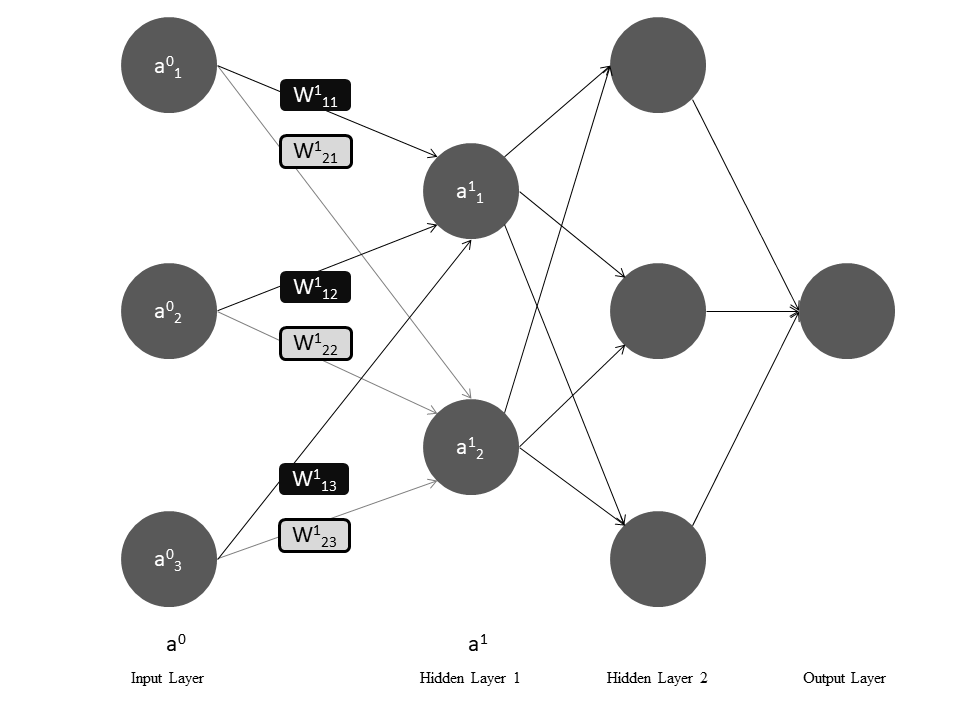
\includegraphics[scale=0.4]{Images/ANN.png}
    \caption{A Fully Connected Neural Network with 2 Hidden Layers. Connections weights are shown between Input layer and Hidden layer 1}
    \label{fig:ANN}
\end{figure}

The \textbf{backpropagation algorithm} changes these weights and biases of the neurons in order to minimize the cost function. Cross Entropy loss is calculated as the cost function for binary classification problems. In order to minimize the cost, we take gradient of the cost (first order derivative) with respect to the parameters of the model and equate it to 0. This indicates the iterative updation of parameters till a minima for the cost is reached, which indicates the optimal model performance.  \\

\textbf{Convolutional Neural Networks} are a class of neural networks which use convolution (or discrete cross-correlation) operation on the input with a kernel/filter at the convolution layer, which is fed to the pooling layer to reduce the dimensionality of the resulting \emph{feature map} by aggregating regions in the neighbouring proximity using mean or maximum values, the output of which is finally fed to a fully connected layer for the prediction of the output. The output of the convolutional layer, or the feature map is given by \\
\begin{center}
    $a_i^{(l)} = f(\sum_{k=1}^K w_i^{(k,l)} * a_{i-1}^{(k)} + b_i^{(l)})$
\end{center}
where the $K$ vectors of length $n_{i-1}$ are input to the $i^{th}$ layer (k=1,2, ..., K) given by $a_{i-1}^{(k)}$, L is the output number of vectors (l=1,2, ...,L) given by $a_i^{(l)}$, $f()$ is the activation function, $*$ is the convolution function, $w_i^{(k,l)}$ is the weight array acting as a filter or kernel and $b_i^{(l)}$ are the bias vector.


\subsection{Recurrent Neural Networks}
Recurrent neural networks are yet another class of NNs which feed the network output back as an input to the network. This allows them to retain information, identify patterns and establish temporal connections, which is suitable for time-series applications.
\begin{figure}[h]
    \centering
    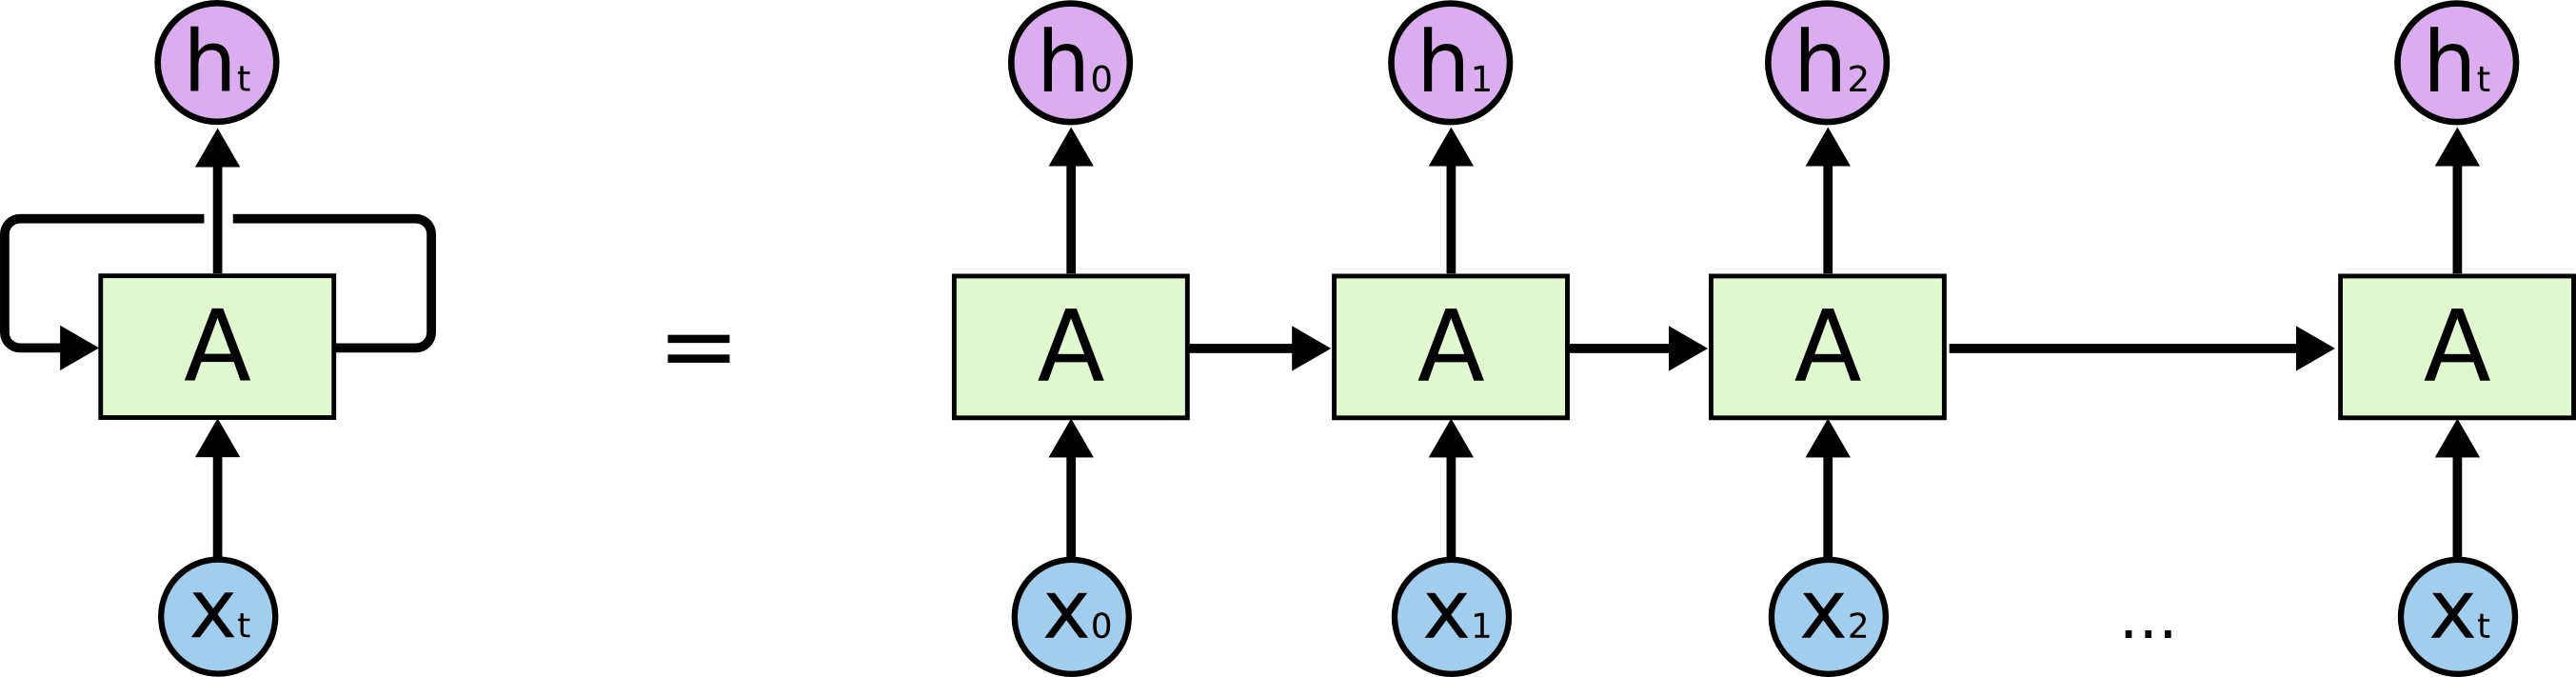
\includegraphics[scale=0.3]{Images/RNNs_1.png}
    \caption{A Recurrent Neural Network. The looped layers are shown unrolled here. \emph{Source}: \href{https://colah.github.io/posts/2015-08-Understanding-LSTMs/}{\textit{Understanding LSTM Networks, Colah 2015}}}
    \label{fig:RNN}
\end{figure}
Long Short Term Memory Networks are a type of gated RNNs that can learn long term dependencies between the data points by removing or adding certain information through the sigmoid gates, controlling this flow of information. There is a Cell-state which flows through the LSTM cells. The information which we need to remove is decided by the first sigmoid gate. The second sigmoid gate in conjecture with $tanh$ of the previous state's output decides what we keep in the cell state. This cell state then factors in with a $tanh$ to the current state's output.
\begin{figure}[h]
    \centering
    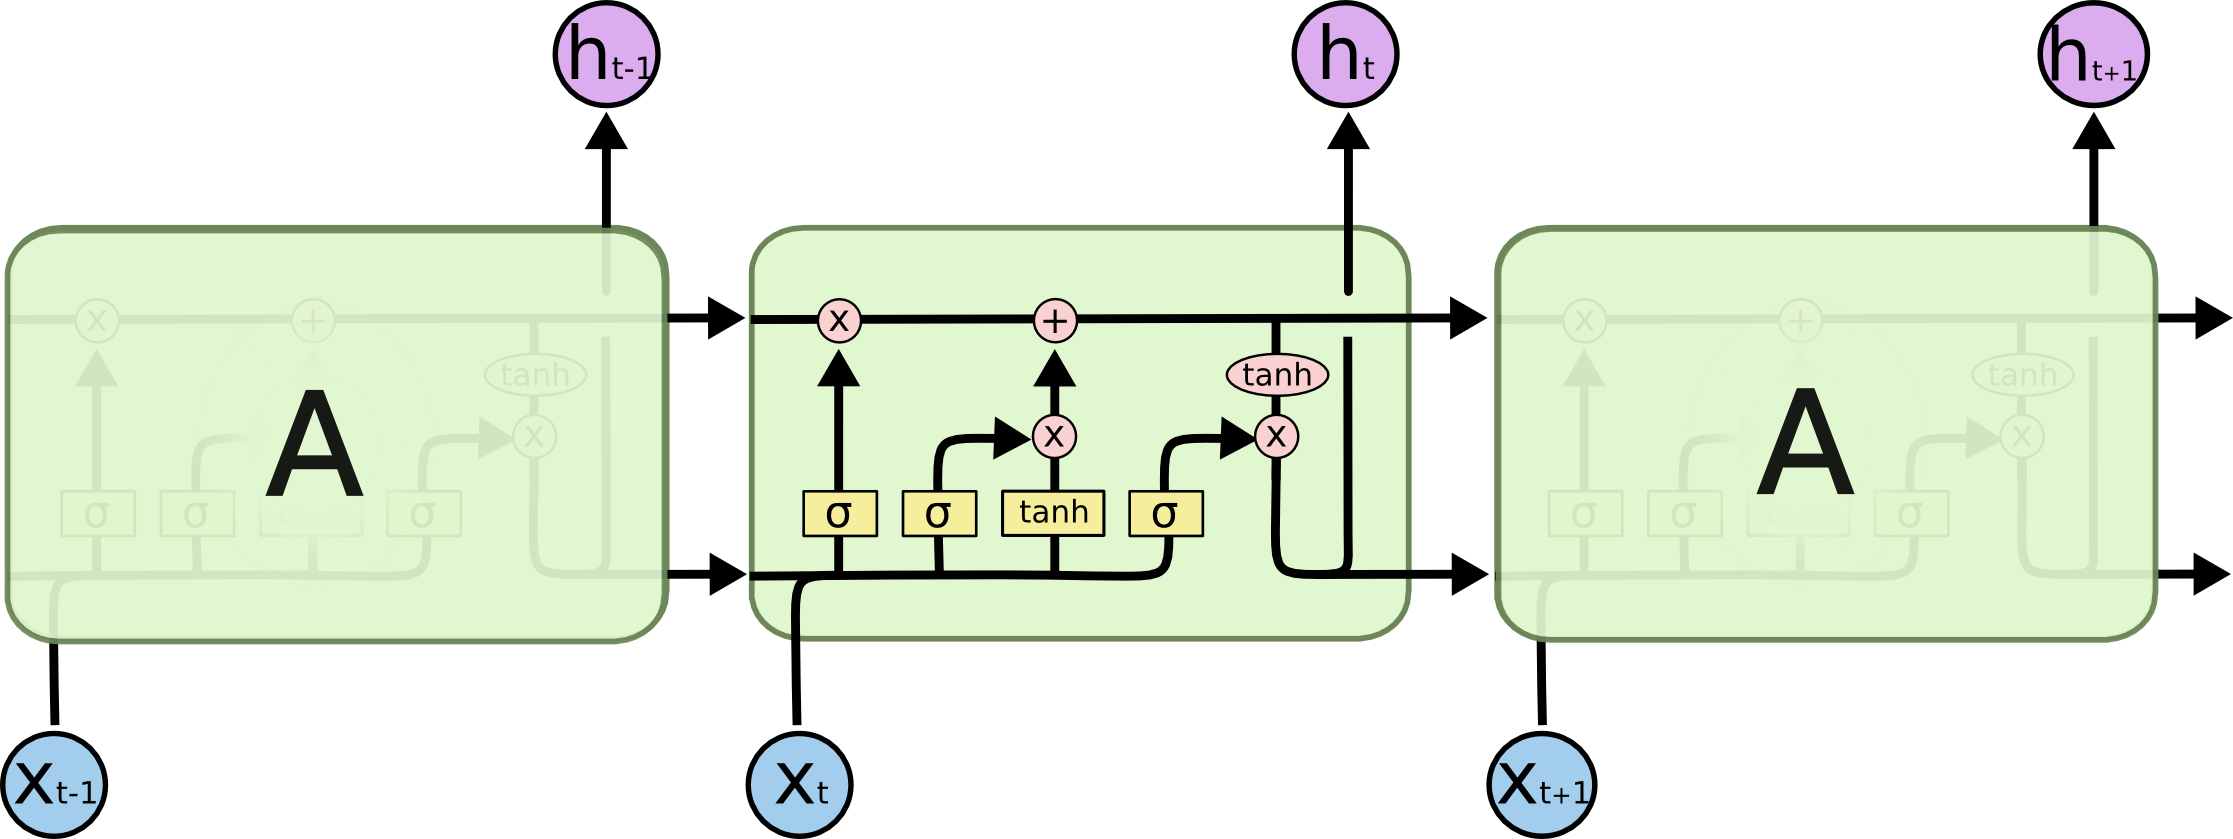
\includegraphics[scale=0.35]{Images/LSTM.png}
    \caption{Simplified architecture of Long Short Term Memory Network. \emph{Source}: \href{https://colah.github.io/posts/2015-08-Understanding-LSTMs/}{\textit{Understanding LSTM Networks, Colah 2015}}}
    \label{fig:LSTM}
\end{figure}
\subsection{Transit Classification}
Transit detection for exoplanets is a field involving space-based high precision photometry. A dip in the stellar flux/brightness indicates a transiting phenomena occuring, or in simpler terms, something is passing between the field of vision from the telescope and the star. We record the stellar lights over a time span and the resulting flux time series is calles a \emph{Light Curve}
\begin{figure}[h]
    \centering
    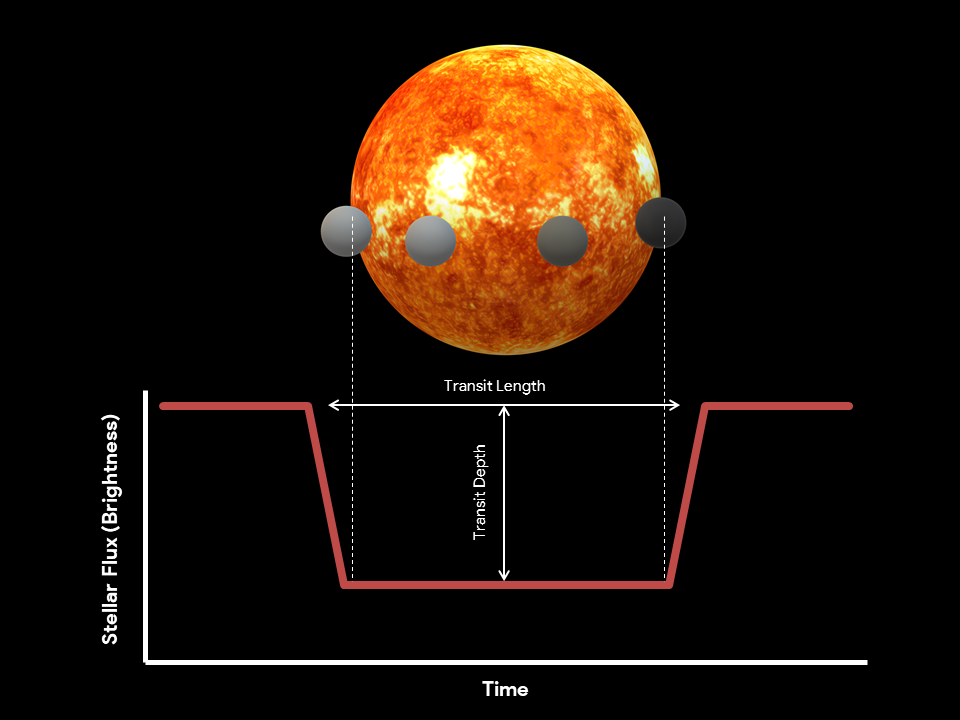
\includegraphics[scale=0.4]{Images/Transit.png}
    \caption{Stellar light curve plotted against a planet transiting it's host star}
    \label{fig:Transit}
\end{figure}







\section{Proposed Methodology}
%What it is: 
%–Describes your hypothesis in detail. (first paragraph)
%–Outlines the steps you will take to prove/disprove your hypothesis (Specific Aims) 
%–Establishes the metrics/benchmarks you will use.
%–Outlines how your time will be allocated. (Timeline!) 
%–Addresses alternatives and contingency plans. 

%What you need to show: 
%–You have a well thought-out and thorough plan of action. 
%–You have clearly defined methods, and metrics for evaluating your results. 
%–You’ve thought about potential delays or obstacles. 
%–Your Aims are appropriate, reasonable, and not interdependent. 


\subsection{Data Required}

\subsection{Time Requirement}



\section{Conclusion}



\begin{thebibliography}{99}

\bibitem{einstein15}
 	\href{http://www.gsjournal.net/old/eeuro/vankov.pdf}{Einstein, A. 1915. \emph{Explanation of the
	Perihelion Motion of Mercury from General Relativity Theory}. Koniglich Preußische Akademie der Wissenschaften (Berlin). Sitzungsberichte: 831-839}
	
\bibitem{oppenheimer39}
	\href{http://journals.aps.org/pr/abstract/10.1103/PhysRev.55.374}{Oppenheimer, J. R. and Volkoff, G. M. 1939. \emph{On Massive Neutron Cores}. Phys. Rev. 55, 374}
	
\bibitem{ligo11}
	\href{https://arxiv.org/pdf/1102.3781v1.pdf}{Abadie, J, and Abbott, B.P. et al. (LIGO Scientific Collaboration and Virgo 	Collaboration). 2011. \emph{Search for gravitational waves from binary black hole inspiral, merger and ringdown}.  		arXiv:1102.3781}

\end{thebibliography}

%%% End document
\end{document}